\documentclass[]{beamer}
\usepackage[spanish]{babel}
\usepackage{mathtools}
\usepackage{amsthm}
\usepackage{xcolor}
\usepackage[most]{tcolorbox} %para encerrar texto en cajas de colores

%%%% Mis macros %%%%

			%% Secciones:
	
			\newtheorem{teo}{\bf Teorema}
			\newtheorem{lema}{\textbf{Lema}}
			\newtheorem{prop}{\bf Proposición}
			\newtheorem{obs}{\bf Observación}
			\newtheorem{dem}{\bf Demostración}
			\newtheorem{cor}{\bf Corolario}
			\newtheorem{defi}{\bf Definición}
			\newtheorem{ej}{\bf Ejemplo}
			\newtheorem{notacion}{\bf Notación}

			
			\theoremstyle{definition}
			\newtheorem{nota}{\bf Nota}

			%% Símbolos matemáticos
			\newcommand*{\QEDA}{\null\nobreak\hfill\ensuremath{\blacksquare}}%
			\newcommand*{\QEDB}{\null\nobreak\hfill\ensuremath{\square}}%
			\newcommand{\TODO}[1]{\textcolor{purple}{#1}}
			\newcommand*{\final}{\null\nobreak\hfill\ensuremath{\diamond}}
			\newcommand{\IR}{\mathbb{R}}
			\newcommand{\IC}{\mathbb{C}}
			\newcommand{\IN}{\mathbb{N}}
			\newcommand{\IZ}{\mathbb{Z}}
			\newcommand{\suma}[3]{\sum\limits_{#1}^{#2}#3} %Sumas y series
			\newcommand{\union}[3]{\bigcup\limits_{#1}^{#2}{#3}} %uniones
			\newcommand{\producto}[3]{\prod_{#1}^{#2}{#3}} %productos
			\newcommand{\limite}[2]{\lim\limits_{#1}{#2}} %límites
			\newcommand{\limsu}[2]{\lim\limits_{#1 \rightarrow \infty }#2_{#1}}
			%para límites de sucesiones
			\newcommand{\Om}{\Omega}
			\newcommand{\cali}[1]{\mathcal{#1}} %Letras caligráficas
			\newcommand{\cont}[2]{$\mathcal{C} [#1, #2]$}
			\newcommand{\integ}[3]{\int_{#1}^{#2}{#3}}
			\newcommand{\ldos}{\mathit{l}^{2}}


			\DeclareMathOperator*{\ameboxplus}{{\boxplus}}







\title{La transformada de Haar-Legendre}
\author{Amélie Bernès}

\usetheme{Madrid}
\useinnertheme{circles}

%\useoutertheme{sidebar} 

\title[PDL]{A study and spectral analysis of the discrete Legendre polynomials} 

\author{Amélie Bernès Carmona \and Moisés Soto Bajo} 

\institute[BUAP]{Benemérita Universidad Autónoma de Puebla \\ \smallskip \textit{ammel.bernes@gmail.com}}

\date[\today]{\today} % Presentation date or conference/meeting name, the optional parameter can contain a shortened version to appear on the bottom of every slide, while the required parameter value is output to the title slide

\begin{document}
\begin{frame}
\titlepage

\end{frame}

%----------------------------------------------------------



% Section; primera parte. Las subsections son
% Motivation and goals
% Construction of the BLD
% Symmetries
% Computation 
% Using representations with the BLD to perform a morphological analysis


%Section: segunda parte
% Motivation of doing a spectral analysis
% Spectral analysis with the DFT
% Spectral analysis using monofrecuential spaces
%
%----------------------------------------------------------
\section{Primera parte}

\begin{frame}
\Huge{
\textbf{
Part One: Definition of the $\cali{L}^{n,k}$
}}
\end{frame}


\begin{frame}
Fixed $n \geq 2$, a signal of dimension $n$ will be represented
with a vector of $\IR^{n}$.

\begin{figure}[h]
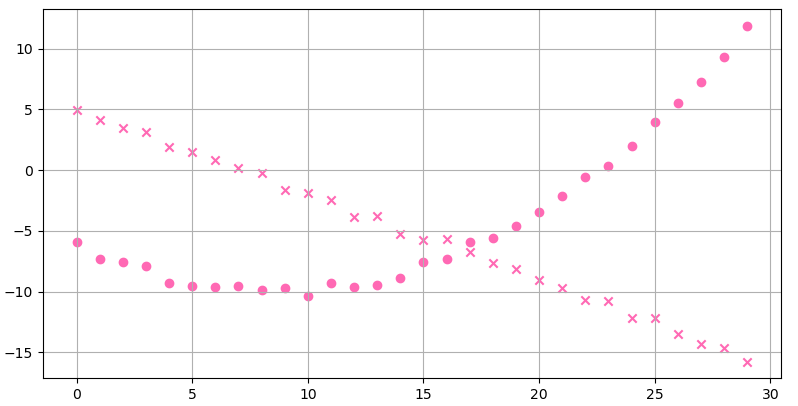
\includegraphics[scale = 0.4]{a}
\end{figure}
We are interested in geometric attributes of the signal, particularly, in
knowing when it behaves like a straight line or like a parabola.

\[
G_{x} := \{ (m, x_{m}) : \hspace{0.2cm} 0 \leq m \leq n-1 \}.
\]
\end{frame}





\begin{frame}
\subsection{Motivation and goals}
Fixed a dimension $n \geq 2$, we are looking for a
basis $$\cali{L}^{n} = \{\cali{L}^{n,k}: \hspace{0.2cm}
0 \leq k \leq n-1\}$$ of $\IR^{n}$ such that
\begin{itemize}
	\item \textcolor{red}{(Size)}
	It is an orthonormal basis of $\IR^{n}$;
\end{itemize}
\[
\forall x\in \IR^{n}: \hspace{0.2cm} x = \suma{k=0}{n-1}{
\langle x, \cali{L}^{n,k} \rangle
}
\]
and
\[
\forall x\in \IR^{n}: \hspace{0.2cm} || x ||^{2} = \suma{k=0}{n-1}{
| \langle x, \cali{L}^{n,k} \rangle |^{2}
}
\]
\begin{itemize}
	\item \textcolor{red}{(Shape)}
	It's possible to establish a simple criteria 
	for the shape of the graph of any signal $x$	
	in terms
	of the coefficients  
	$\langle x, \cali{L}^{n,k} \rangle$ of it with respect
	to $\cali{L}^{n}$.
\end{itemize}


\end{frame}
%----------------------------------------------------------


\begin{frame}
Let $x = (x_{m})_{m=0}^{n-1} \in \IR^{n}$.
\TODO{Define al operador de discr. puntual. y a los espacios Wk}
\begin{align*}
x \textit{ is affine} & \Leftrightarrow &
x = (a)
\end{align*}

Likewise, 
\begin{center}
$x$ is constant iff $x \in W_{n,0}$
\end{center}
and
\begin{center}
$x$ is cuadratic iff $x \in W_{n,2}$.
\end{center}
\end{frame}

\begin{frame}
\frametitle{Some properties of the subspaces $W_{n,k}$}
\section{Some properties of the subspaces $W_{n,k}$}
\begin{prop}
		Let $n \geq 2$, $0 \leq k \leq n-1$. Let $W_{n,k}$
		be as.
		\begin{itemize}
		\item $dim(W_{n,k}) = k+1$, 
		\item $\forall 0 \leq i \leq n-2$: $W_{n, i} \subseteq W_{n, i+1}$,
		\item $\IR^{n} = W_{n, n-1}$
		\item Let $\cali{P} = \{ t_{j} := t_{0}+ hj : 
		\hspace{0.2cm} 0 \leq j \leq n-1 \}$ be a uniform mesh of $n$
		points. For all $x \in \IR^{n}$ and all $0 \leq i \leq n-1$, $x \in W_{n,i}$
		if and only if there exists a polynomial $g(x)$ of degree at most
		$i$ such that $x = \Omega_{n, \cali{P}}(g)$.
		\end{itemize}
\end{prop}
\end{frame}



\begin{frame}

The belonging to a subspace $W_{n,k}$
determines the shape of the graph of a signal $x$.

\begin{figure}[h]
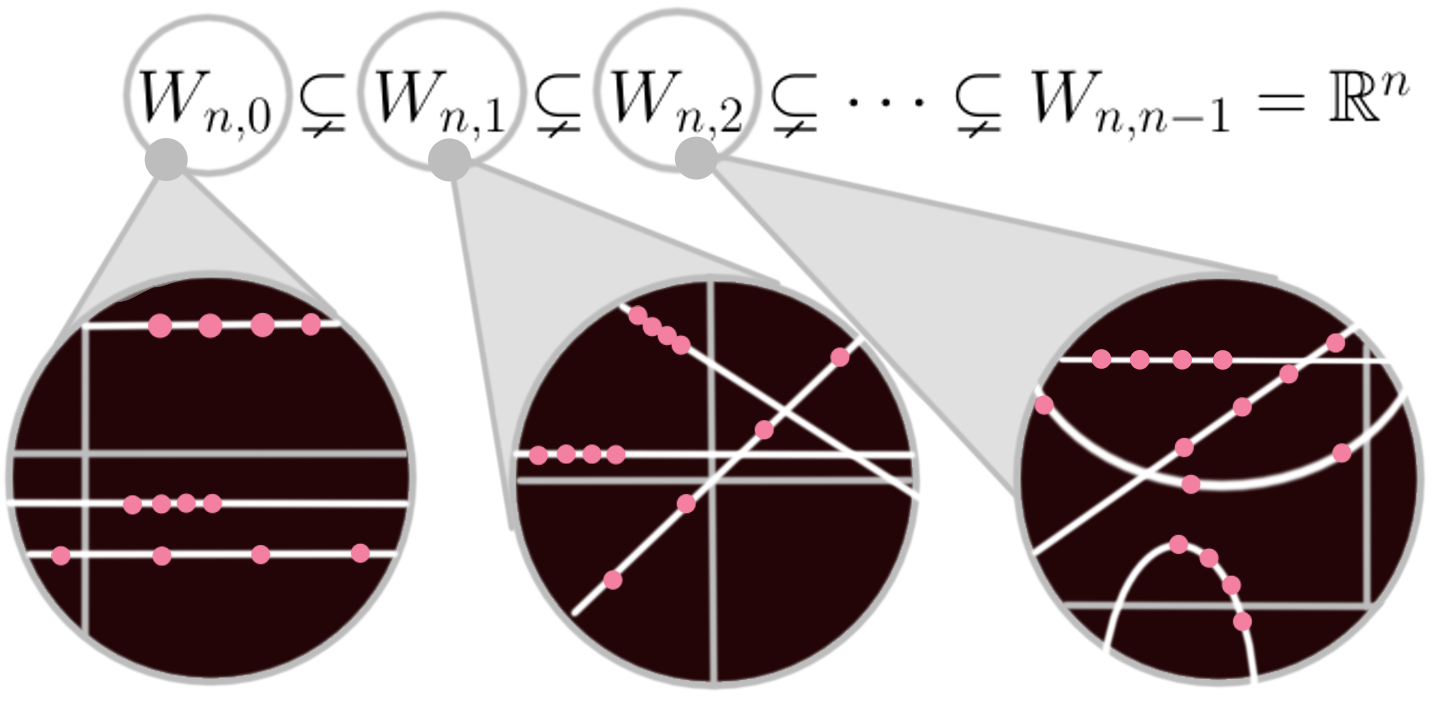
\includegraphics[scale = 1]{nuevas_lupas}
\end{figure}
\end{frame}


\begin{frame}
\frametitle{The definition of the degree of a finite signal}


\begin{prop}
Let $n \geq 2$ and $\cali{P}$ be a uniform mesh of $n$ points.
The function 
\[
\Omega_{n, \cali{P}}: \IR_{n-1}[t] \longrightarrow \IR^{n}
\]
is an isomorphism of $\IR-$vector spaces.
\end{prop}

Notice that the mesh $\cali{P}$ is fixed at the beginning.
Can we find two meshes $\cali{P}$ and $\tilde{\cali{P}}$
and two polynomials $f, \tilde{f}$ of degrees
$0 \leq \partial(f) < partial(\tilde{f}) \leq n-1$
such that
\[
\Omega_{n, \cali{P}}(f) = x = \Omega_{n, \tilde{\cali{P}}}(\tilde{f}) ?
\]
\end{frame}

\begin{frame}
What is sure is that we can not assure uniqueness if
we remove the restriction in the degrees of the polynomials. 
\begin{figure}[h]
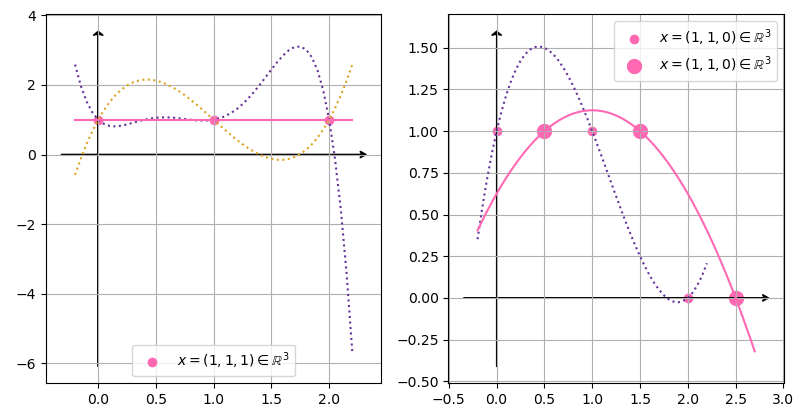
\includegraphics[scale = 0.5]{25Nov_1}
\end{figure}
\end{frame}

\begin{frame}
\begin{prop}
Let $n \geq 2$, $x \in \IR^{n}$. If $\cali{P}$ and $\tilde{\cali{P}}$
are uniform meshes of $n$ points and $f, \tilde{f} \in \IR_{n-1}[t]$ 
are such that
\[
\Omega_{n, \cali{P}}(f) = x = \Omega_{n, \tilde{\cali{P}}}(\tilde{f}).
\]
then $\partial(f) = \partial(\tilde{f})$.
\end{prop}

\begin{defi}
Let $n \geq 2$ and $x \in \IR^{n}$. If $f \in \IR_{n-1}[t]$
and $\cali{P}$ is a uniform mesh of $n$ points such that
$x = \Omega_{n, \cali{P}}(f)$, then 
\[
\partial(x) := \partial(f)
\]
\end{defi}
\end{frame}


\begin{frame}
\frametitle{Relationship between the degree of a signal and the spaces $W_{n,k}$}
Let $n \geq 2$ and $x \in \IR^{n}$.
\begin{itemize}
\item $x$ has degree 0 iff $x \in W_{n,0}$
\item for all $1 \leq i \leq n-1$, $x$ has degree $i$ iff
$x \in W_{n,i}$
\end{itemize}

Thus, $W_{n,k}$ is the space of signals of degree $k$. \\
Let's find orthonormal basis for those spaces.

\end{frame}


\begin{frame}
\begin{figure}[h]
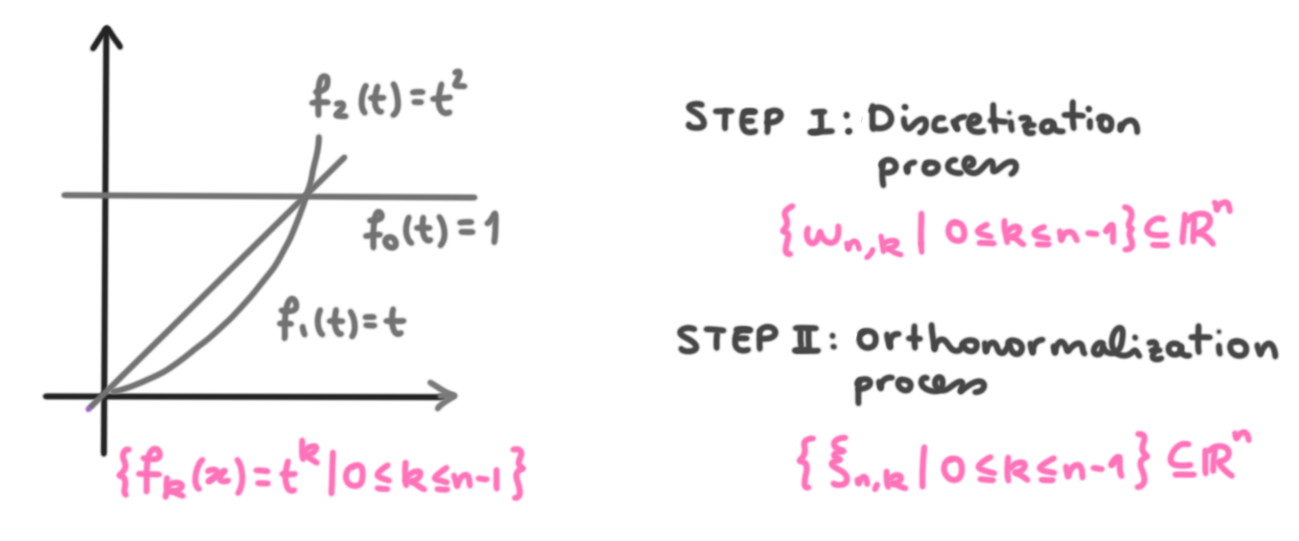
\includegraphics[scale = 1]{1}
\end{figure}
\end{frame}

\begin{frame}
\begin{figure}[h]
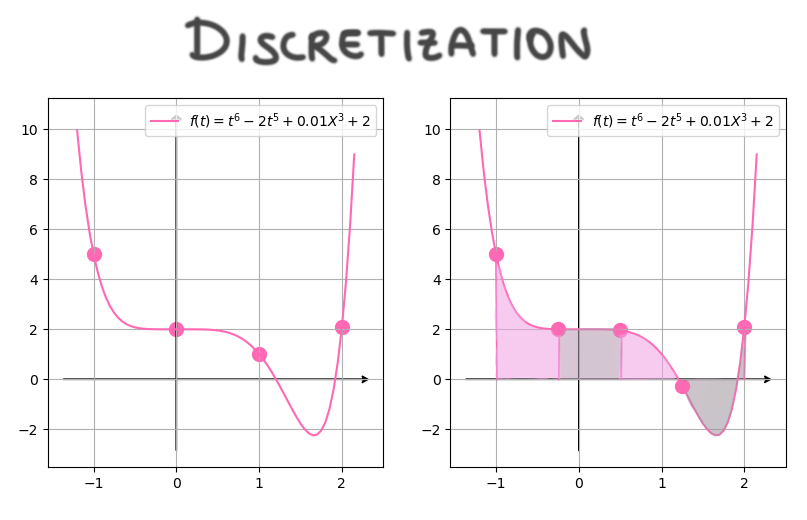
\includegraphics[scale = 1.4]{discretization}
\end{figure}
\end{frame}

\begin{frame}
\begin{figure}[h]
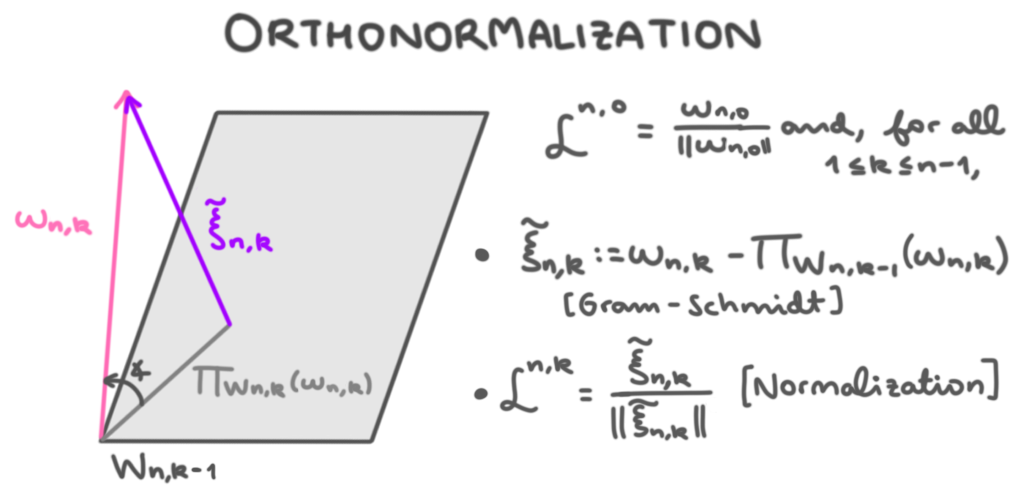
\includegraphics[scale = 1.4]{orthonorm}
\end{figure}
\end{frame}

\begin{frame}
Thus, if $x \in \IR^{n}$, 
\begin{itemize}
	\item $x$ has degree $k$ if and only if $x \in W_{n,k}$
	(binary answer)
	\item We can actually measure how far apart 
	$x$ is from $W_{n,k}$, thus \textbf{we can measure how much
	$x$ is far away from the property ``having degree $k$''}
\end{itemize}
\end{frame}

\begin{frame}
\frametitle{How to measure the distance to a subspace?}
\begin{figure}[h]
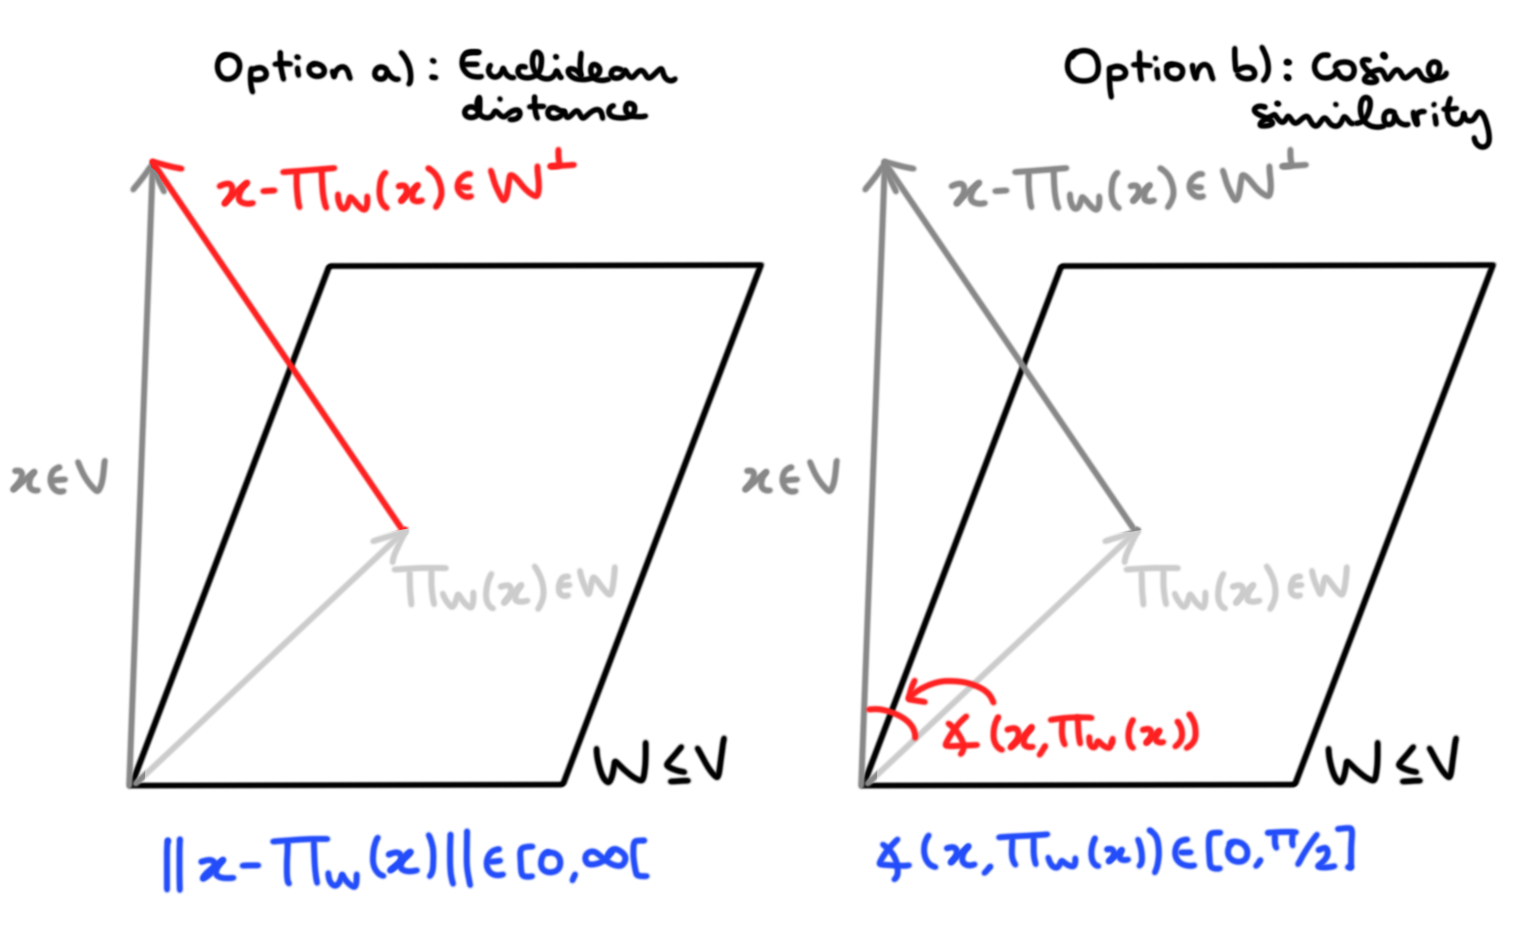
\includegraphics[scale = 0.9]{18Sept_1}
\end{figure}
\end{frame}

\begin{frame}
\frametitle{Why cosine similarity is better for us?}
Answer: it is, as well as the
shape of the graph of a signal, 
invariant under scalar multiplication.

\begin{figure}[h]
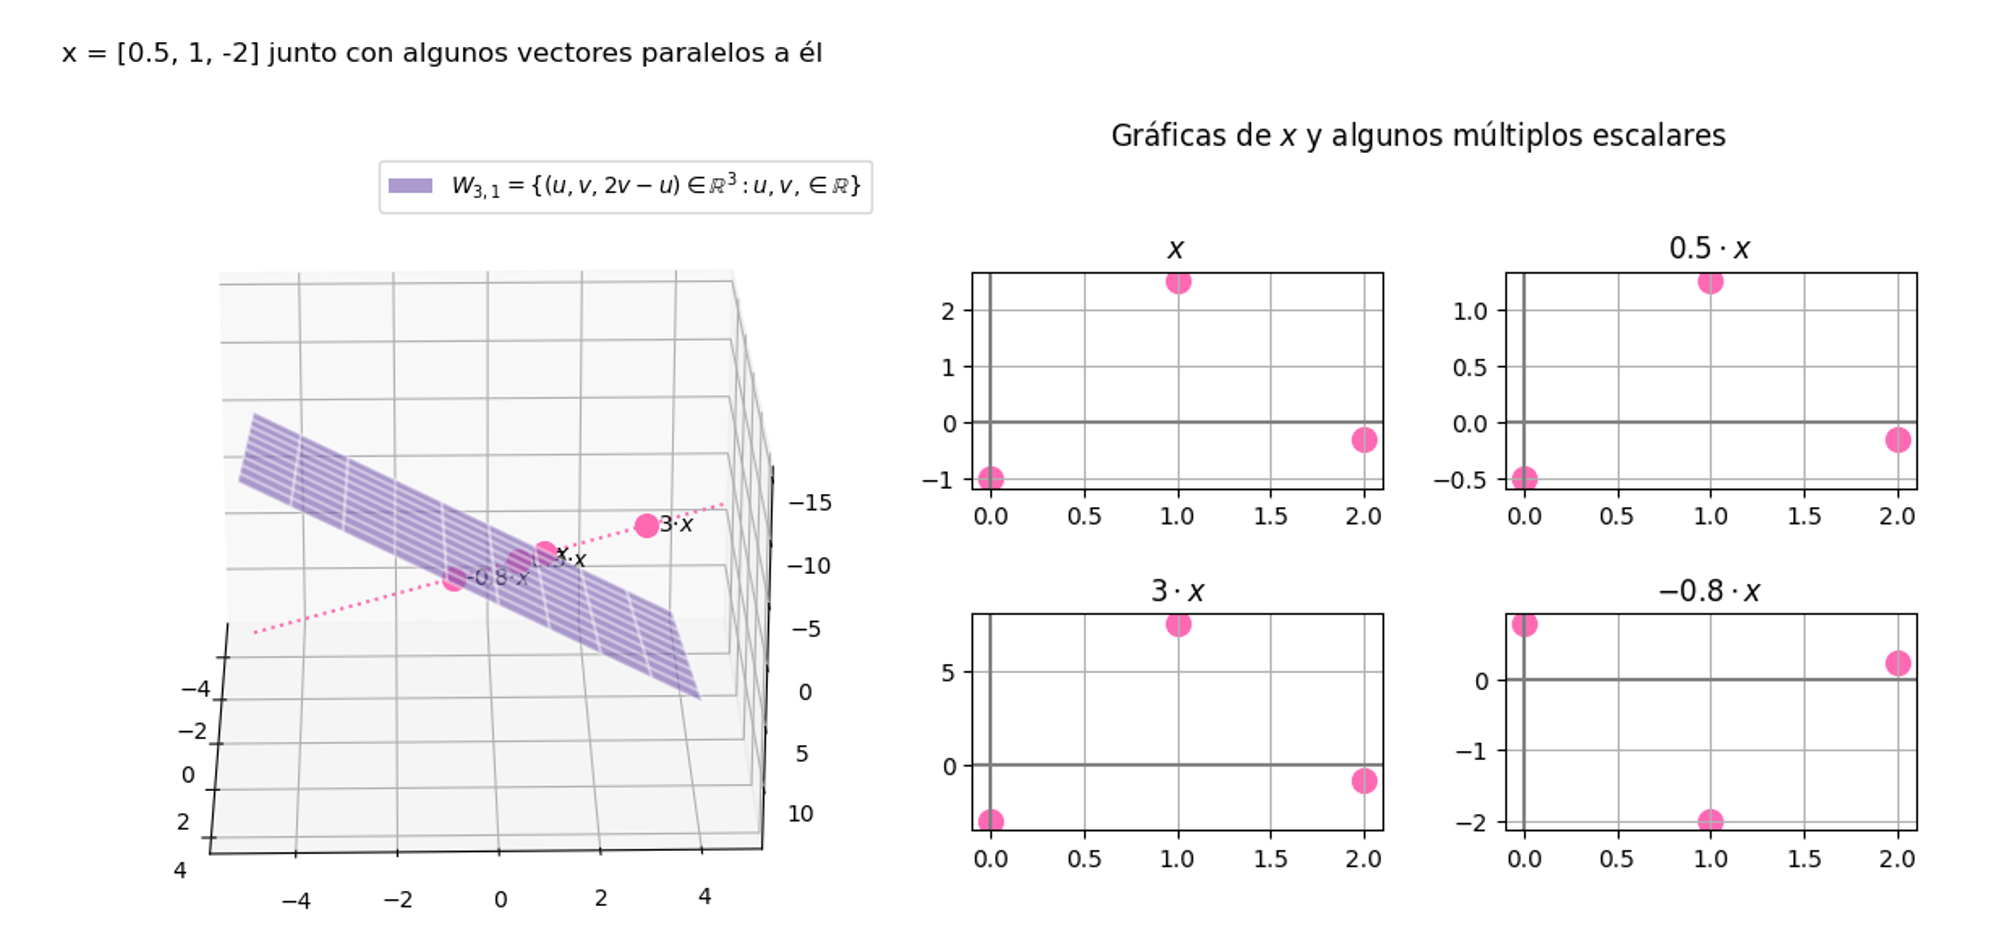
\includegraphics[scale = 0.15]{borrador}
\end{figure}
\end{frame}


\begin{frame}
\frametitle{Using coefficientes with respect to $\cali{L}^{n}$ to make a morphological analysis}
\begin{figure}[h]
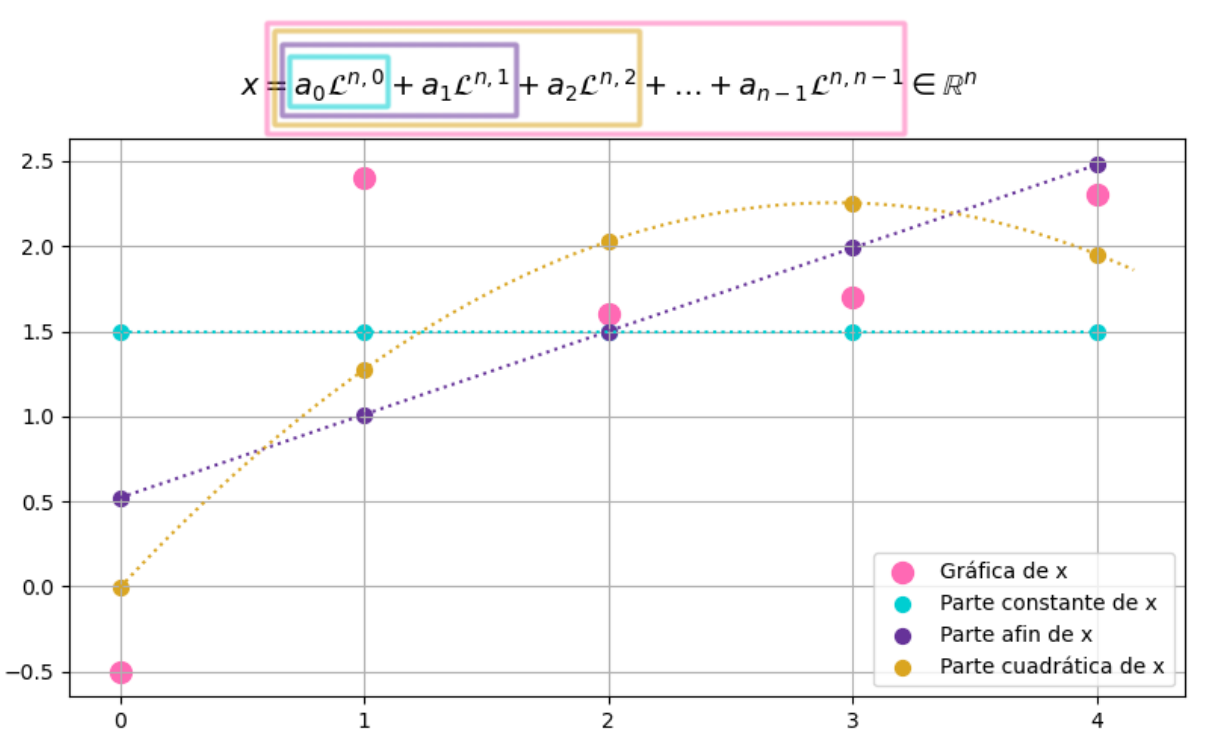
\includegraphics[scale = 0.35]{abee}
\end{figure}
\end{frame}



\begin{frame}
Let $x = \suma{i=0}{n-1}{a_{i}\cali{L}^{n,i}} \in \IR^{n}$.
\begin{itemize}
	\item $x$ is approximately constant iff $a_{0}^{2} \sim ||x||^{2}$ 
	\item $x$ is approximately affine iff $a_{0}^{2} + a_{1}^{2} \sim ||x||^{2}$ 
	\item $x$ is approximately cuadratic iff $a_{0}^{2} + a_{1}^{2} + a_{2}^{2} \sim ||x||^{2}$ 
\end{itemize}

In general, $x$ has nearly degree $k$ iff the energy 
$||x||^{2}$ is concentrated in the first $k$ coefficients $a_{k}$.

\TODO{poner fórmulas}
\end{frame}

\begin{frame}
\frametitle{Example in $\IR^{3}$}
\begin{figure}[h]
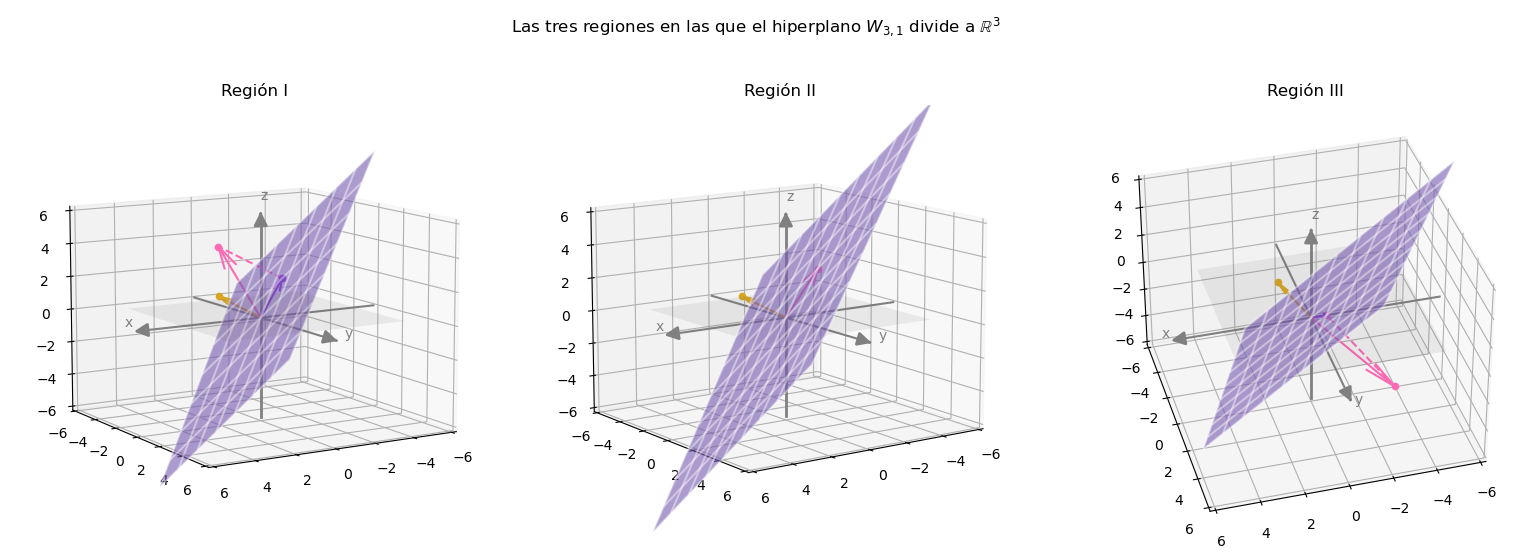
\includegraphics[scale = 0.3]{2Dic_4}
\end{figure}
\end{frame}

\begin{frame}
\begin{figure}[h]
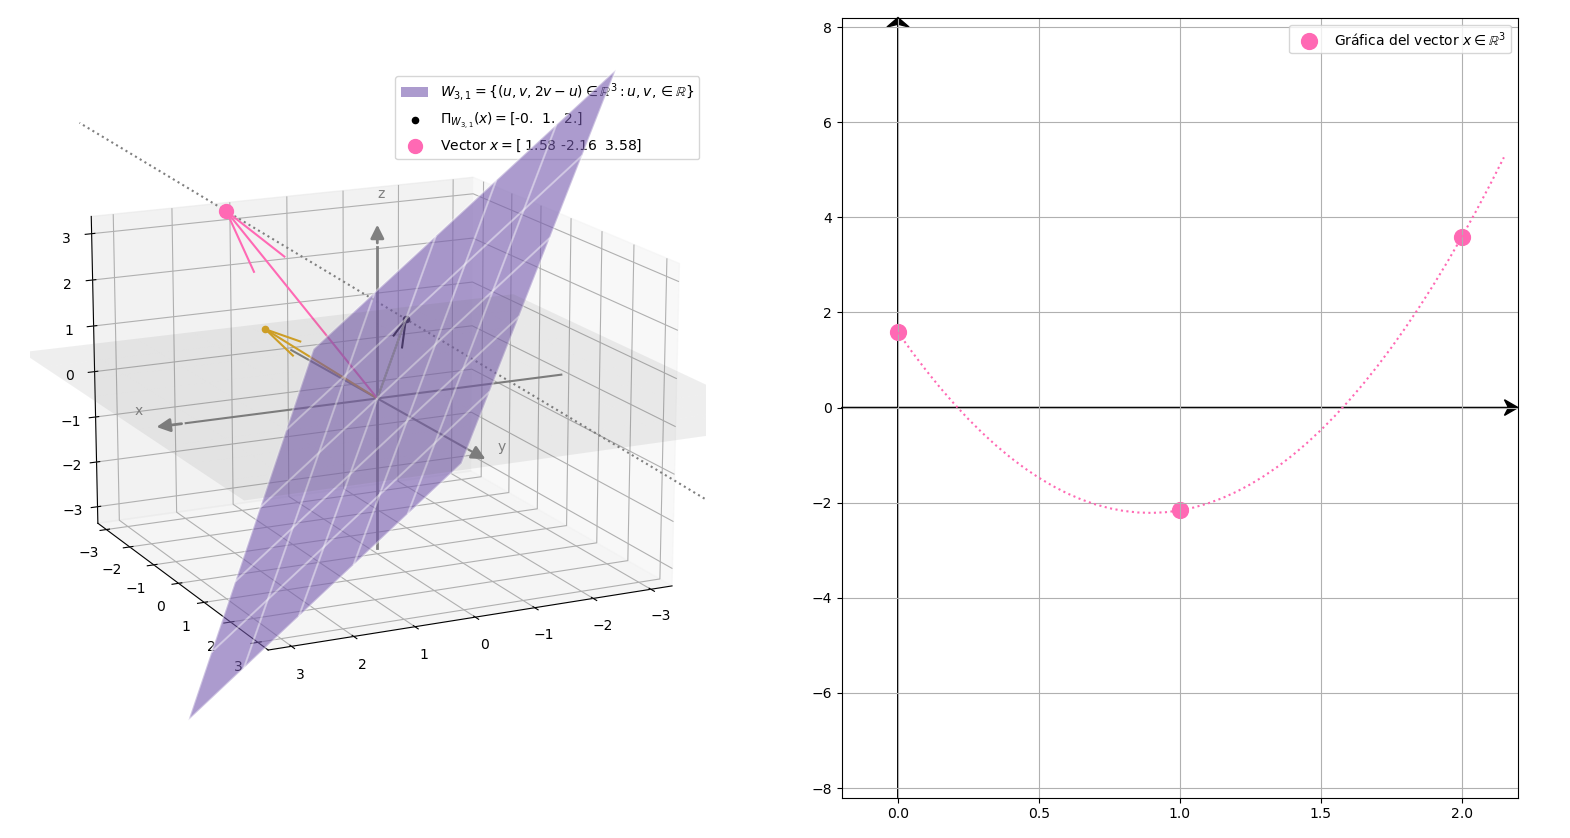
\includegraphics[scale = 0.3]{6Dic_0}
\end{figure}
\end{frame}

\begin{frame}
\begin{figure}[h]
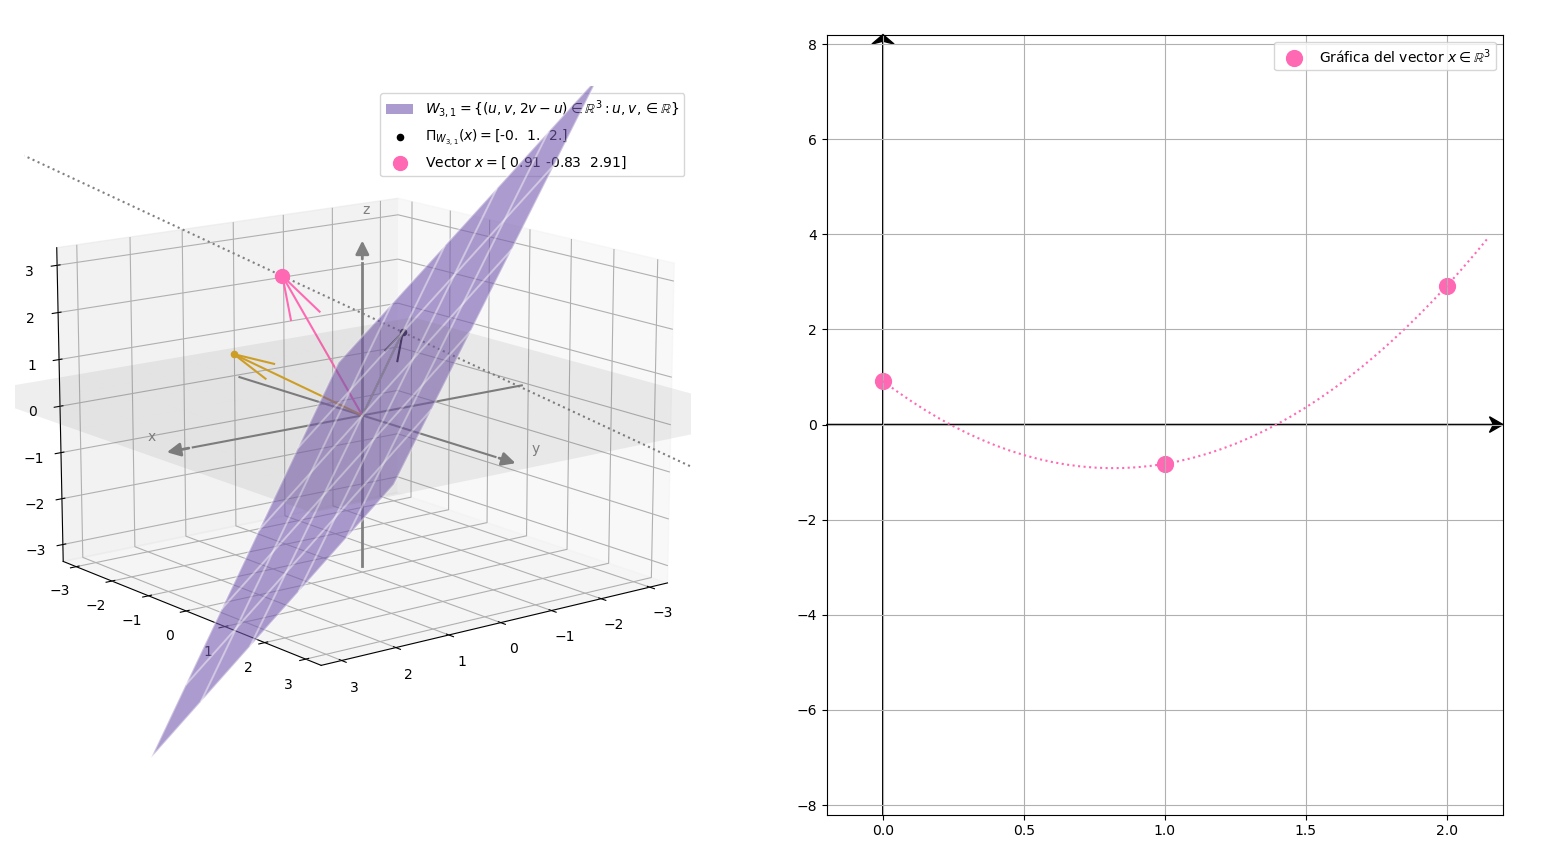
\includegraphics[scale = 0.3]{6Dic_1}
\end{figure}
\end{frame}

\begin{frame}
\begin{figure}[h]
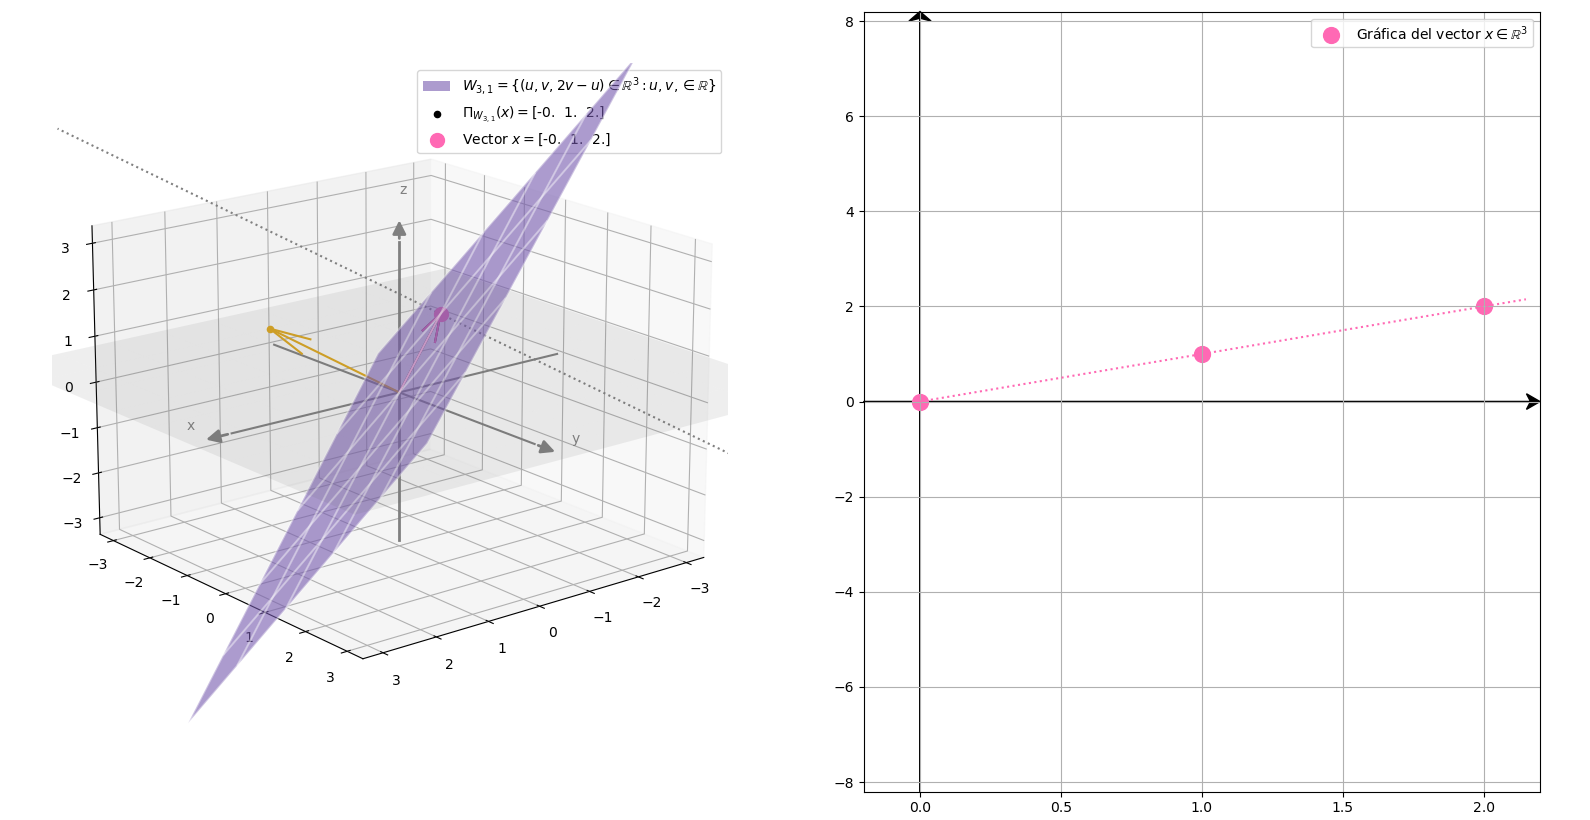
\includegraphics[scale = 0.3]{6Dic_2}
\end{figure}
\end{frame}

\begin{frame}
\begin{figure}[h]
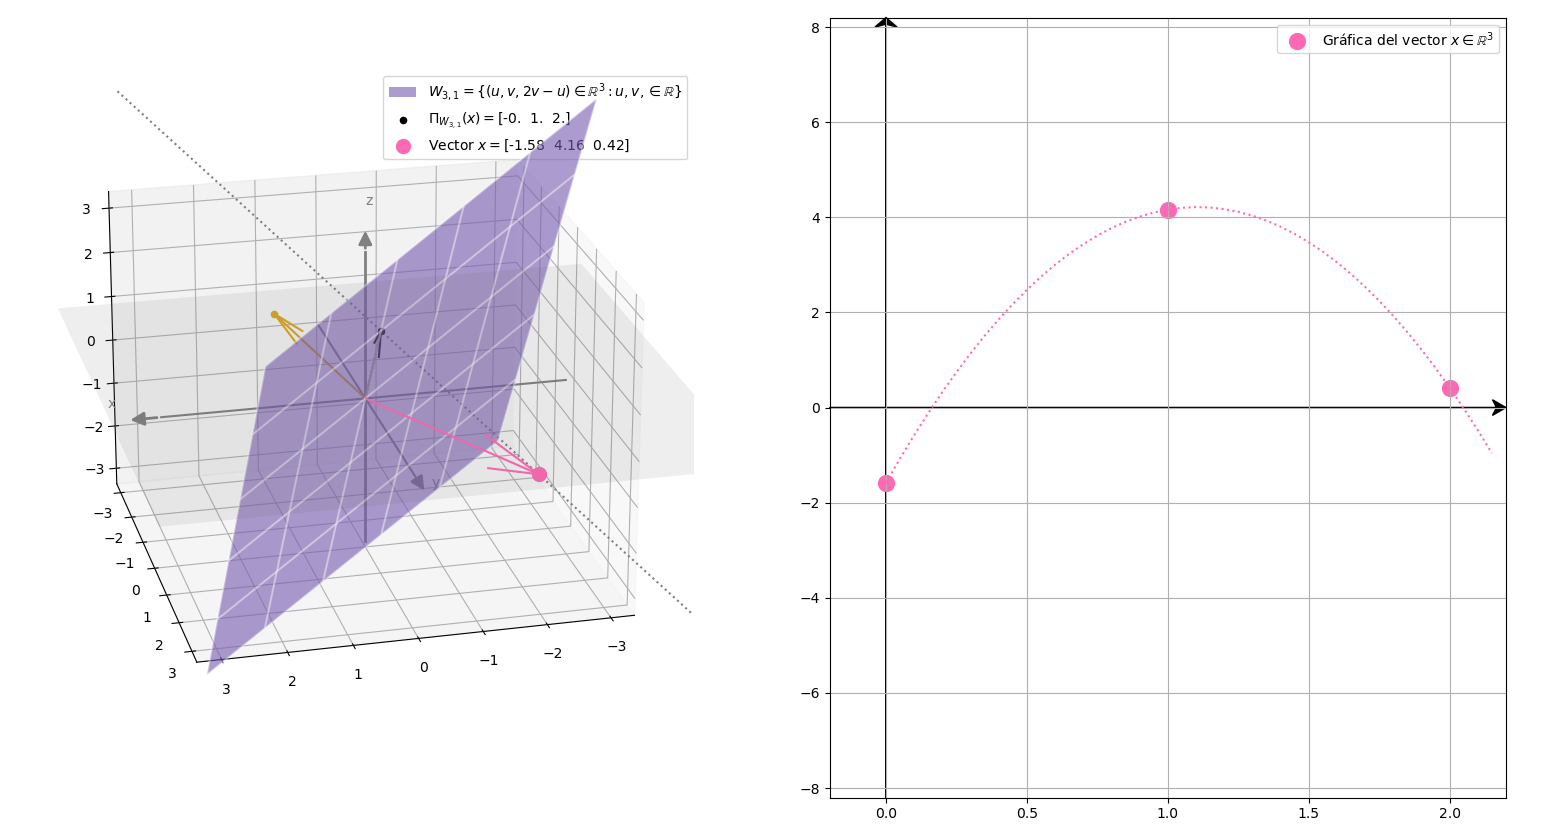
\includegraphics[scale = 0.3]{6Dic_3}
\end{figure}
\end{frame}

\begin{frame}
\begin{figure}[h]
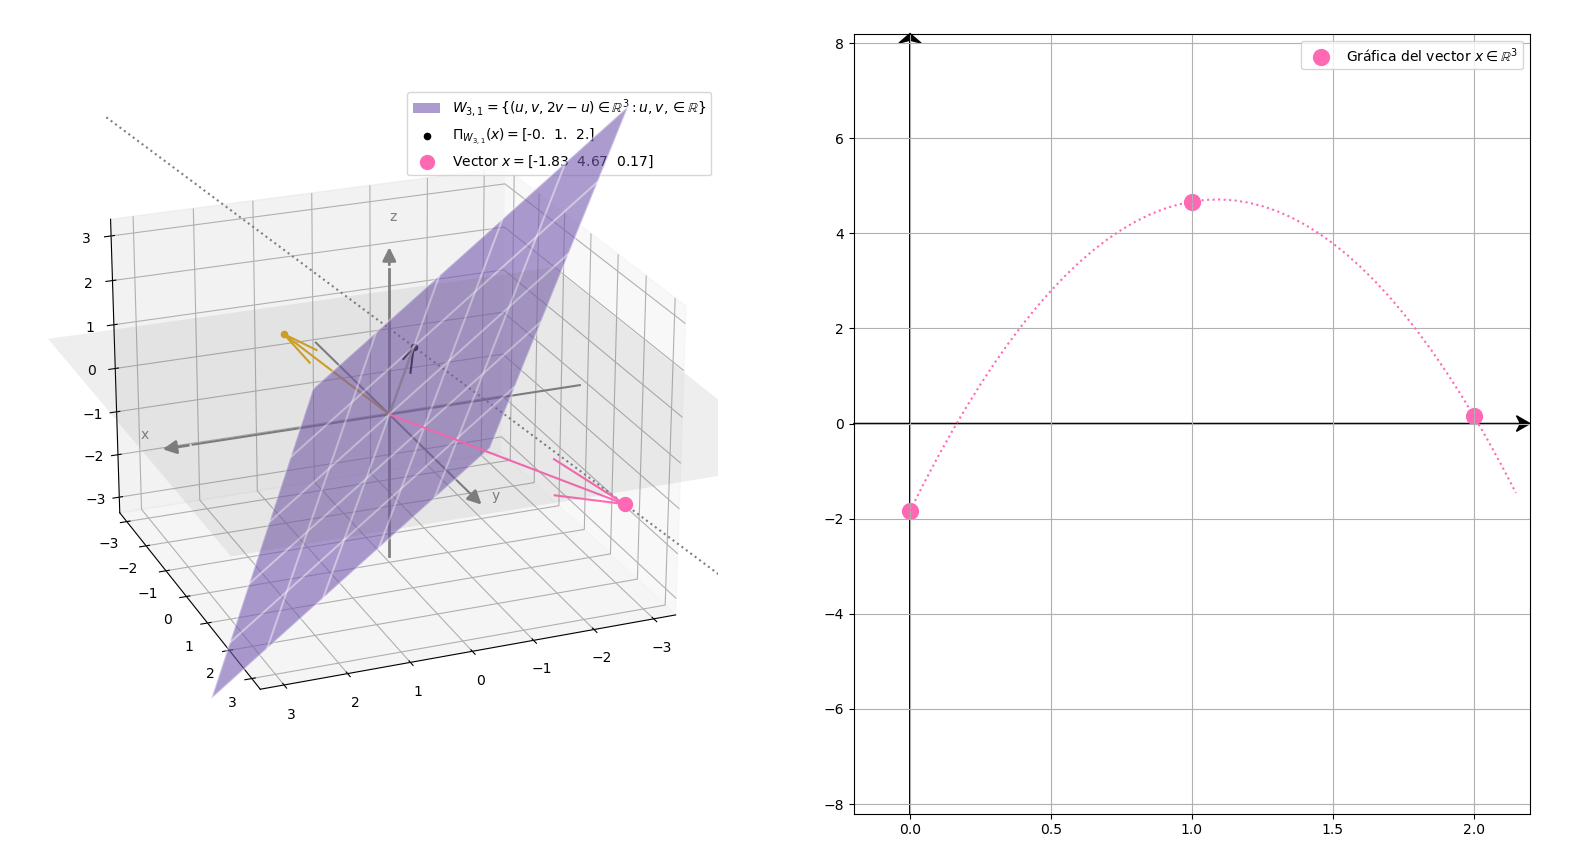
\includegraphics[scale = 0.3]{6Dic_4}
\end{figure}
\end{frame}


\begin{frame}
\frametitle{Relationship with the minimum square approximation method}
a
\end{frame}


\begin{frame}
\Huge{
\textbf{
Part Two: Spectral analysis
}}
\end{frame}

\end{document}


